%%%%%%%%%%%%%%%%%%%%%%%%%%%%%%%%%%%%%%%%%%%%%%%%%%%%%%%%%%%%%%%%%%%%%%%%
% Preamble
%%%%%%%%%%%%%%%%%%%%%%%%%%%%%%%%%%%%%%%%%%%%%%%%%%%%%%%%%%%%%%%%%%%%%%%%
\documentclass[11pt]{article}
%
% Packages and other includes
% Pagination
\usepackage[letterpaper, margin=1.25in]{geometry}
%
% Fonts
\usepackage[T1]{fontenc} % best for Western European languages
\usepackage{lmodern} % Latin Modern instead of CM
\usepackage{textcomp} % required to get special symbols
%
% Math
\usepackage{amsmath, amssymb}
\usepackage{braket}
%
% Graphics, floats, tables
\usepackage{graphicx, xcolor, float, array}
\usepackage{subcaption}
%
% Hyperlinks
\usepackage{hyperref}
%
% Bibliography
\usepackage[style=numeric, sorting=none, backend=biber]{biblatex}
\addbibresource{references.bib}
%
% Revision (see Makefile)
%\input{revision.tex}
%
% Definitions and settings
% Paragraph indent and spacing
\setlength{\parskip}{0.4\baselineskip}
\setlength{\parindent}{0in}
%
% Math mode version of "r" column type (requires array package)
\newcolumntype{R}{>{$}r<{$}}
%
%comments
\newcommand{\brian}[1]{{\color{orange} #1}}
% Title, authors, date
\title{\textbf{Is TPSS an TPSSh better for TPAA calculations?}}
\author{Thanh Huynh and Brian Nguyen}
\date{11/27/2020 -- 01/10/2021 }
%
%
%%%%%%%%%%%%%%%%%%%%%%%%%%%%%%%%%%%%%%%%%%%%%%%%%%%%%%%%%%%%%%%%%%%%%%%%
% Main document
%%%%%%%%%%%%%%%%%%%%%%%%%%%%%%%%%%%%%%%%%%%%%%%%%%%%%%%%%%%%%%%%%%%%%%%%
%

\begin{document}

\maketitle

\section{Introduction}

\brian{Mention big picture -> lissoclimide project; follow-up to the
  previous report}

A potent cytotoxin, called chlorolissoclimide, was discovered
in the sea squirt and could potentially be useful in cancer therapeutics
or other medication. This chemical induces cell death by obstructing
production of proteins. An interesting ribosome-drug interaction was
revealed to form a halogen-pi bond however, characteristics of the bond
are still unknown. Researching this specific interaction could help with
creating new cancer therapeutics or improving medication.

Following up the previous report, random phase approximation (RPA) was
chosen to be used with different functionals. The TPSS and TPSSh
functionals may describe the halogen-pi bond more accurately than PBE.
To investigate which functional performs better, the X40 test set serves
as a benchmark for TPSS, TPSSh, and PBE calculations.  


\section{Methods}

Based on the previous report, the 3-4 extrapolation of the RIRPA
correlation energy was a good balance between efficiency and accuracy.
The X40 Test Set was used to benchmark the method's accuracy for 
noncovalent interactions involving halogens. The test set contains 40
complexes with despersion, induction, dipole-dipole, stack, hydrogen
bond, halogen bond, and halogen-pi bond interations.

To conserve time, a set of eight complexes from the X40 test set were
chosen based on error from the previous report to study basis set
convergences. Calculations were computed with basis sets def2-QZVP,
cc-pVTZ, and cc-pVQZ. The RPA energies were computed based on converged
orbitals from TPSS and TPSSh and resolution of identity (RI) was included
to improve efficiency. The Hartree Exact Exchange (HXX) total energy and
RIRPA correlation energy were recorded from the supermolecule and monomers
of each complex to compute interaction energies. The interaction energies
from the selected complexes were extrapolated...

\section{Results}

\begin{figure}[hbpt]
  \centering
  \begin{subfigure}{\textwidth}
    \center
    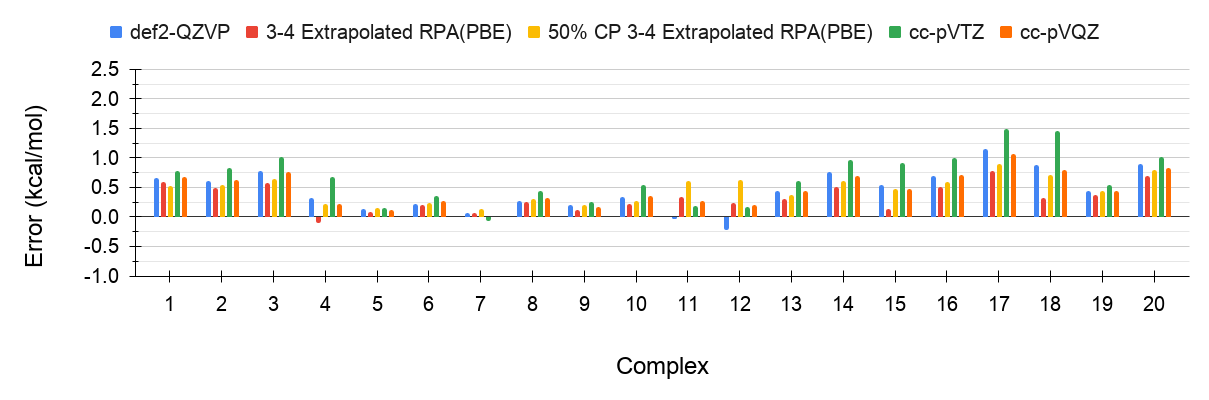
\includegraphics[scale=0.35]{def2-QZVP_1.png}
    \label{fig:def2-QZVP_1}
  \end{subfigure}
  \begin{subfigure}{\textwidth}
    \center
    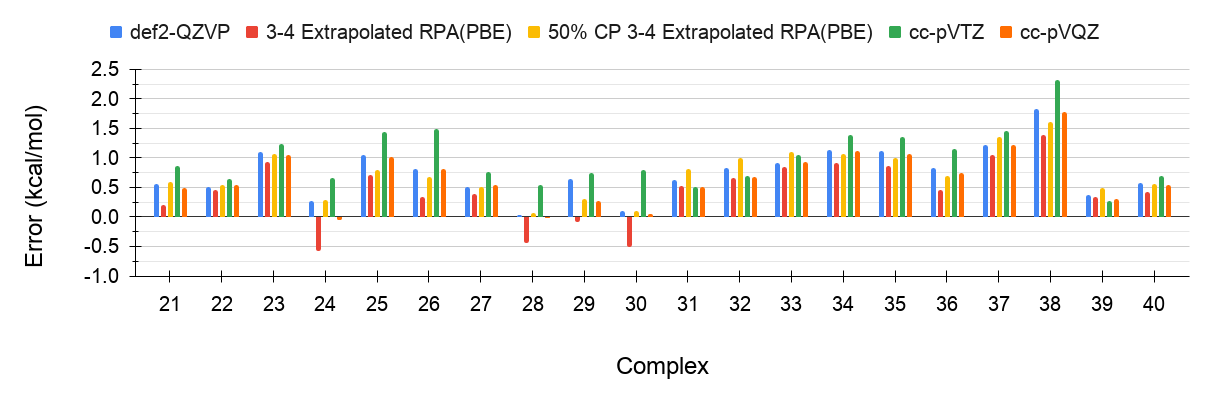
\includegraphics[scale=0.35]{def2-QZVP_2.png}
    \label{fig:def2-QZVP_2}
  \end{subfigure}
  \caption{The binding energy errors (kcal/mol) for X40 test set computed
    for RPA(PBE) methods with basis functions def2-QZVP, cc-pVTZ, and
    cc-pVQZ. Negative sign indicates overbinding.}
  \label{fig:def2-QZVP Error}
\end{figure}

\begin{figure}[hbpt]
  \centering
  \begin{subfigure}{.5\textwidth}
    \centering
    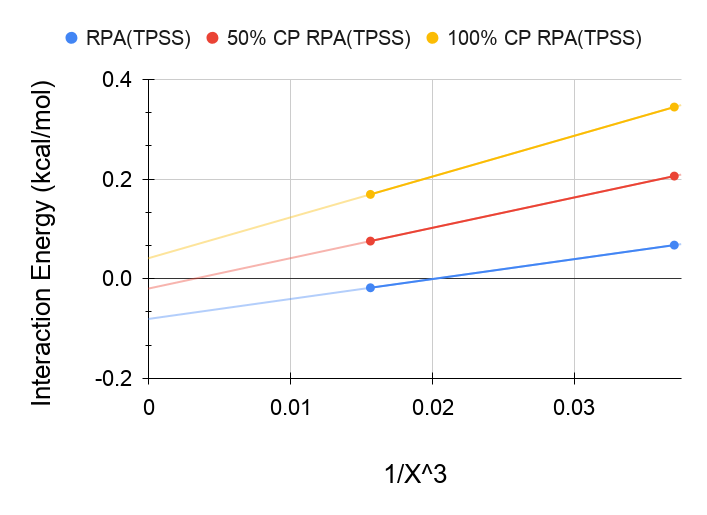
\includegraphics[scale=0.3]{tpss-1.png}
    \caption{RPA(TPSS)}
    \label{fig:tpss_1}
  \end{subfigure}%
  \begin{subfigure}{.5\textwidth}
    \centering
    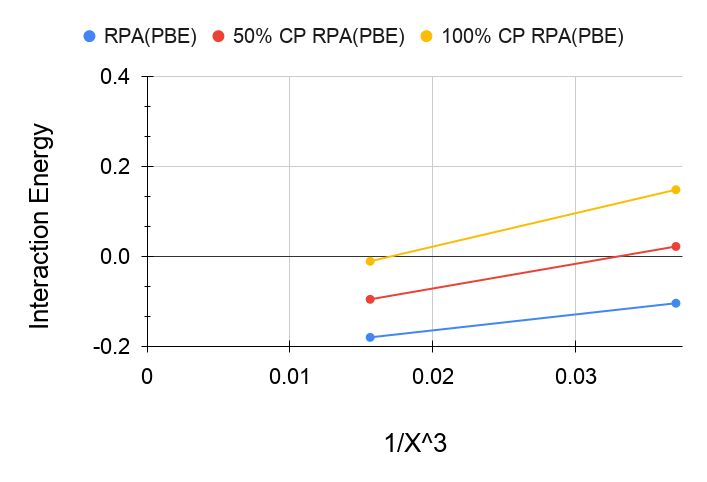
\includegraphics[scale=0.3]{tpssh-1.png}
    \caption{RPA(TPSSh)}
    \label{fig:tpssh_1}
  \end{subfigure}
  \caption{Basis sets convergence plot for RPA(TPSS) and RPA(TPSSh) is
    presented for complex 1. Complex 1 contains dispersion interaction
    with fluorine.}
  \label{fig:complex_1}
\end{figure}

\begin{figure}[hbpt]
  \centering
  \begin{subfigure}{.5\textwidth}
    \centering
    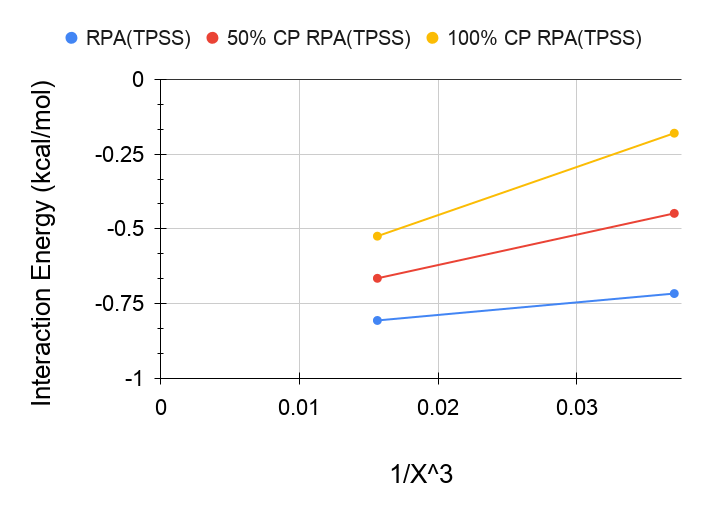
\includegraphics[scale=0.3]{tpss-8.png}
    \caption{RPA(TPSS)}
    \label{fig:tpss_8}
  \end{subfigure}%
  \begin{subfigure}{.5\textwidth}
    \centering
    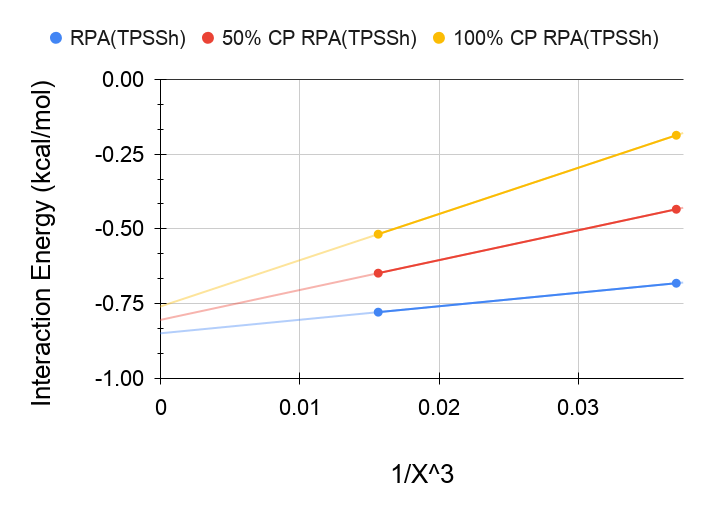
\includegraphics[scale=0.3]{tpssh-8.png}
    \caption{RPA(TPSSh)}
    \label{fig:tpssh_8}
  \end{subfigure}
  \caption{Basis sets convergence plot for RPA(TPSS) and RPA(TPSSh) is
    presented for complex 8. Complex 8 contains induction interactions
    with chlorine.}
  \label{fig:complex_8}
\end{figure}

\begin{figure}[hbpt]
  \centering
  \begin{subfigure}{.5\textwidth}
    \centering
    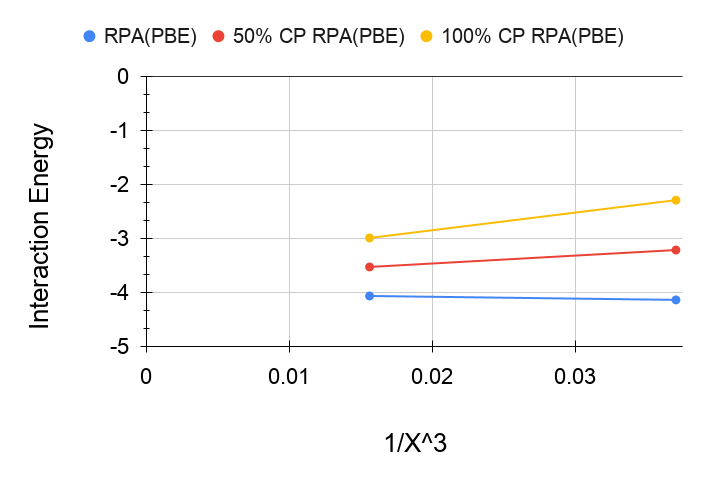
\includegraphics[scale=0.3]{tpss-11.png}
    \caption{RPA(TPSS)}
    \label{fig:tpss11}
  \end{subfigure}%
  \begin{subfigure}{.5\textwidth}
    \centering
    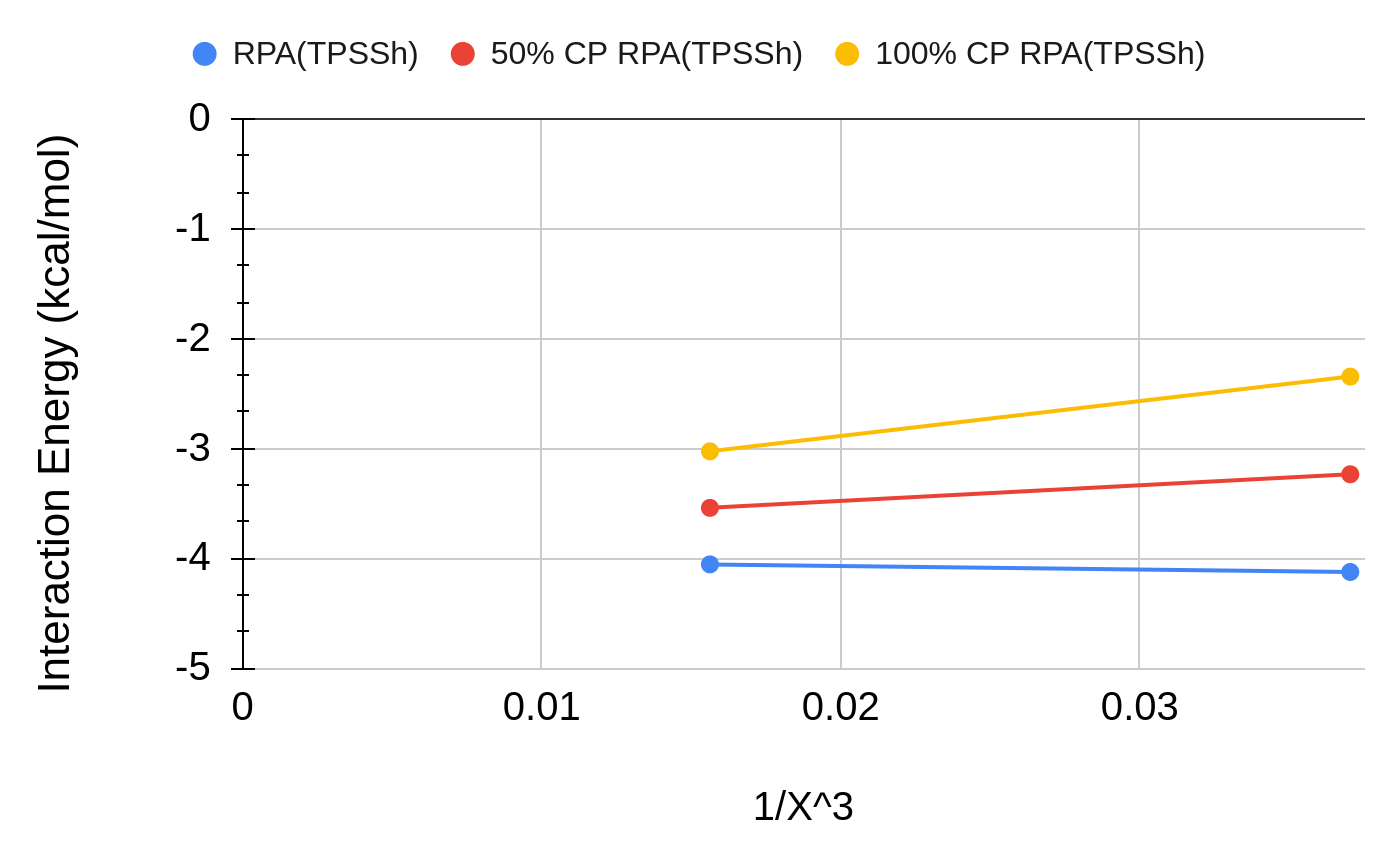
\includegraphics[scale=0.3]{tpssh-11.png}
    \caption{RPA(TPSSh)}
    \label{fig:tpssh_11}
  \end{subfigure}
  \caption{Basis sets convergence plot for RPA(TPSS) and RPA(TPSSh) is
    presented for complex 11. Complex 11 contains stack interactions with
    fluorine.}
  \label{fig:complex_11}
\end{figure}

\begin{figure}[hbpt]
  \centering
  \begin{subfigure}{.5\textwidth}
    \centering
    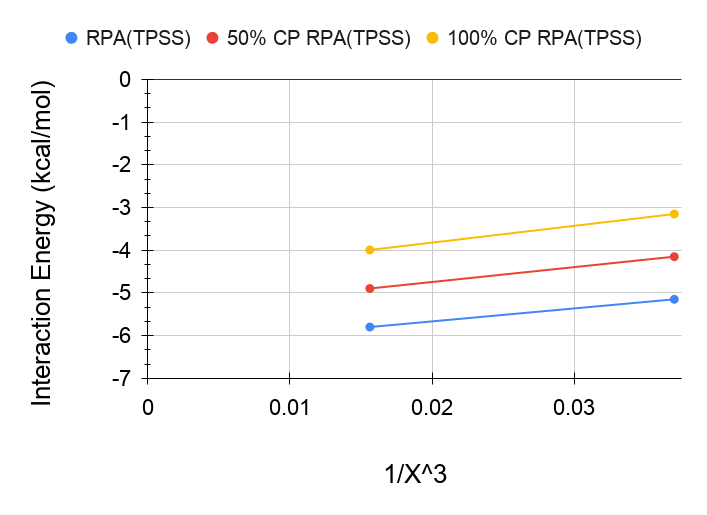
\includegraphics[scale=0.3]{tpss-24.png}
    \caption{RPA(TPSS)}
    \label{fig:tpss_24}
  \end{subfigure}%
  \begin{subfigure}{.5\textwidth}
    \centering
    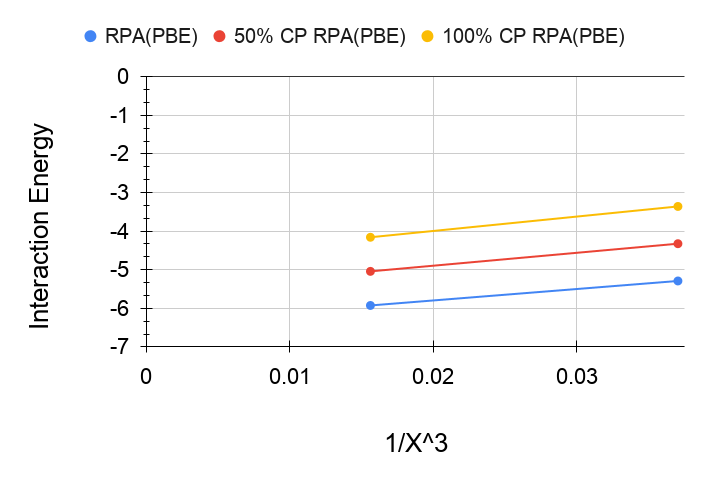
\includegraphics[scale=0.3]{tpssh-24.png}
    \caption{RPA(TPSSh)}
    \label{fig:tpssh_24}
  \end{subfigure}
  \caption{Basis sets convergence plot for RPA(TPSS) and RPA(TPSSh) is
    presented for complex 24. Complex 24 contains halogen bonding with
    iodine.}
  \label{fig:complex_24}
\end{figure}

\begin{figure}[hbpt]
  \centering
  \begin{subfigure}{.5\textwidth}
    \centering
    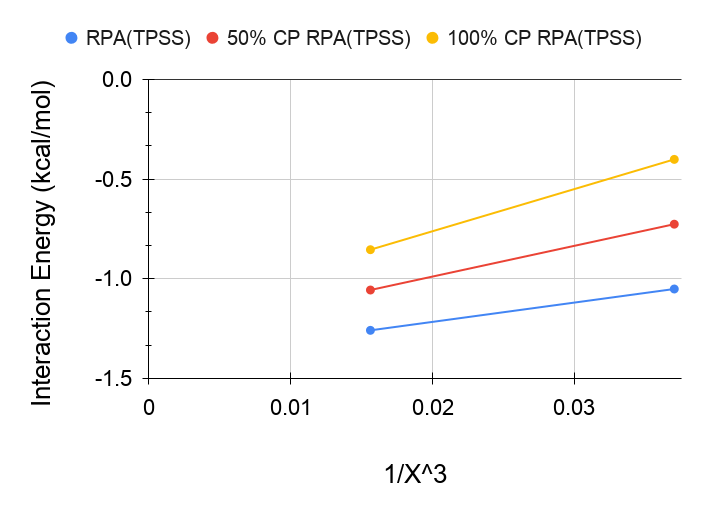
\includegraphics[scale=0.3]{tpss-27.png}
    \caption{RPA(TPSS)}
    \label{fig:tpss_27}
  \end{subfigure}%
  \begin{subfigure}{.5\textwidth}
    \centering
    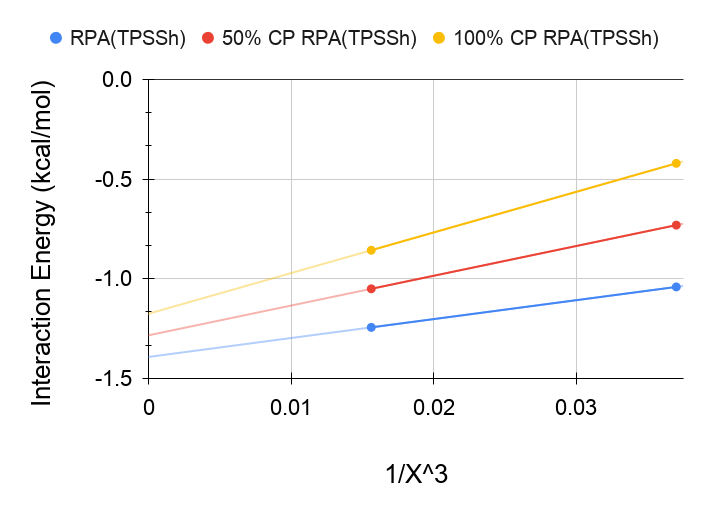
\includegraphics[scale=0.3]{tpssh-27.png}
    \caption{RPA(TPSSh)}
    \label{fig:tpssh_27}
  \end{subfigure}
  \caption{Basis sets convergence plot for RPA(TPSS) and RPA(TPSSh) is
    presented for complex 27. Complex 27 contains halogen-pi bonding
    with bromine.}
  \label{fig:complex_27}
\end{figure}

\begin{figure}[hbpt]
  \centering
  \begin{subfigure}{.5\textwidth}
    \centering
    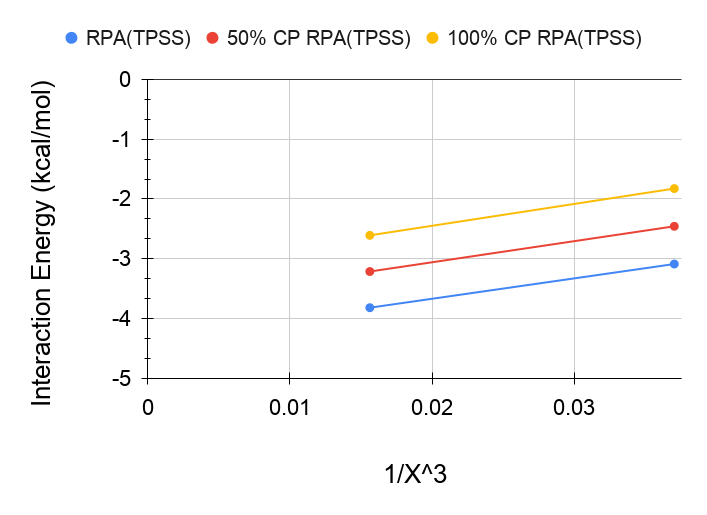
\includegraphics[scale=0.3]{tpss-30.png}
    \caption{RPA(TPSS)}
    \label{fig:tpss_30}
  \end{subfigure}%
  \begin{subfigure}{.5\textwidth}
    \centering
    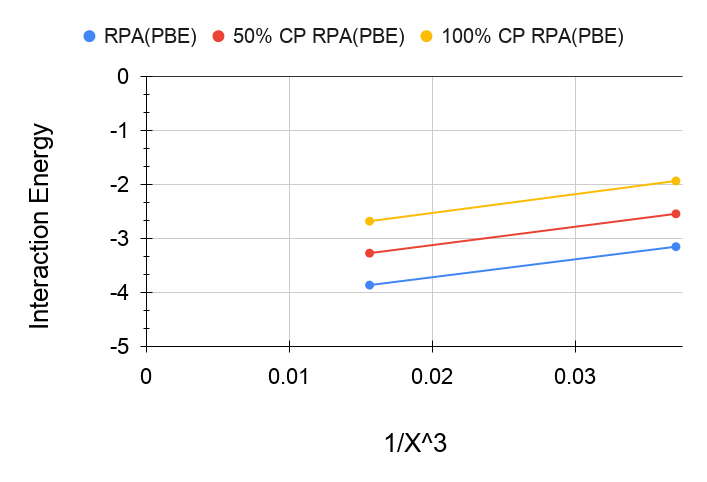
\includegraphics[scale=0.3]{tpssh-30.png}
    \caption{RPA(TPSSh)}
    \label{fig:tpssh_30}
  \end{subfigure}
  \caption{Basis sets convergence plot for RPA(TPSS) and RPA(TPSSh) is
    presented for complex 30. Complex 30 contains halogen-pi bonding
    with iodine.}
  \label{fig:complex_30}
\end{figure}

\begin{figure}[hbpt]
  \centering
  \begin{subfigure}{.5\textwidth}
    \centering
    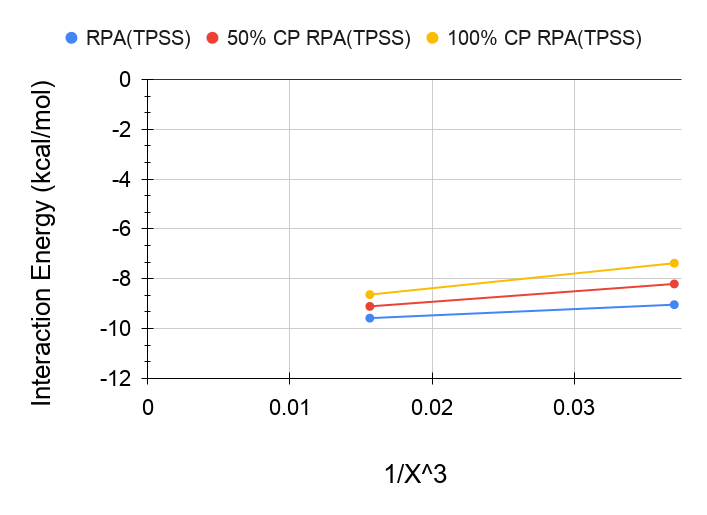
\includegraphics[scale=0.3]{tpss-38.png}
    \caption{RPA(TPSS)}
    \label{fig:tpss_38}
  \end{subfigure}%
  \begin{subfigure}{.5\textwidth}
    \centering
    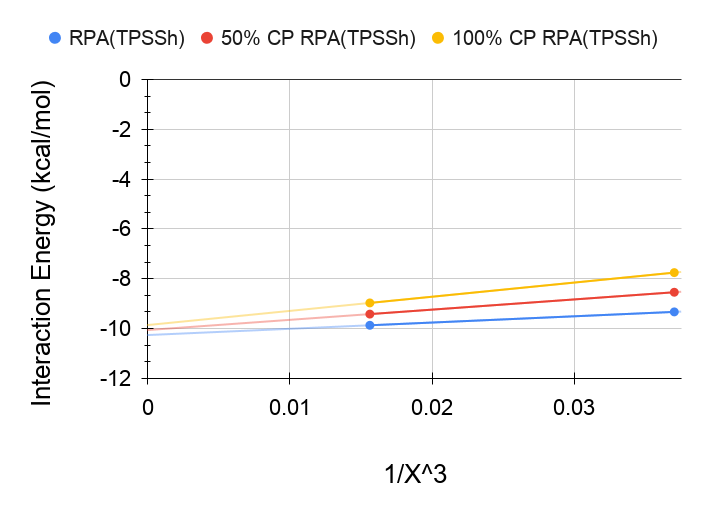
\includegraphics[scale=0.3]{tpssh-38.png}
    \caption{RPA(TPSSh)}
    \label{fig:tpssh_38}
  \end{subfigure}
  \caption{Basis sets convergence plot for RPA(TPSS) and RPA(TPSSh) is
    presented for complex 38. Complex 38 contains hydrogen bonding with
    chlorine.}
  \label{fig:complex_38}
\end{figure}



\brian{yada yada see Fig. \ref{fig:<name>}}
This section states the main new results of the current
reporting period. These results could be presented, e.g., in the form of
equations, figures, tables, and text. Negative results are just as
important as positive ones and should be carefully reported. Use a
balanced tone avoiding over- and understatement. 

Sometimes, it is helpful to separate statement of the results and
discussion, although a strict separation of the two is often
impossible. A separate discussion section may be appropriate if you are
proposing a speculative rationale or if several interpretations of your
results are possible. If you have no new results at all, this is the
place to explain why. 

\section{Conclusions}


This section should answer the following questions:
What is the significance of your results for the question, problem, or
hypothesis posed in the introduction? What, if any, are the
implications in the broader context of the research area laid out in the
second paragraph of the introduction? 

A second paragraph should discuss any conclusions for your future work. 
Is there a need to change your approach or your priorities? What remains
to be done to reach the goals stated in the first section? 

\printbibliography

\end{document}
